\documentclass{book}
\usepackage{color}
\usepackage{colortbl}
\usepackage{graphicx}
\usepackage{subfigure}
\usepackage{hyperref}

\definecolor{lightBrown}{rgb}{0.5,0.2,0.2}
\definecolor{darkBrown}{rgb}{0.5,0,0}
\definecolor{darkBlue}{rgb}{0,0,0.5}
\definecolor{deepBlue}{rgb}{0,0,0.5}
\definecolor{lightGrey}{rgb}{0.9,0.9,0.9}
\definecolor{darkGrey}{rgb}{0.3,0.3,0.3}
\definecolor{lightYellow}{rgb}{1.0,1.0,0.9}
\definecolor{darkGreen}{rgb}{0.0,0.3,0.0}
\definecolor{lightGreen}{rgb}{0.95,1.0,0.95}
\definecolor{darkDarkBrown}{rgb}{0.1,0.1,0.0}
\definecolor{BrickRed}{rgb}{0.7,0.3,0.4}

\newcommand{\csection}[1]{\textcolor{darkBrown}{\section{#1}}}
\newcommand{\cchapter}[1]{\textcolor{lightBrown}{\chapter{#1}}}
\newcommand{\ccaption}[1]{\textcolor{deepBlue}{\caption{#1}}}
\newcommand{\mm}[1]{\textcolor{darkDarkBrown}{$#1$}}
\newcommand{\param}[1]{\fcolorbox{darkGreen}{lightGreen}{\textcolor{darkGreen}{#1}}}
\newcommand{\warning}[1]{
\begin{center}
\begin{tabular}{|c>{\columncolor{lightGrey}}p{4in}|}
    \hline
\includegraphics[height=0.1in,angle=45]{warning.eps} & \textcolor{red}{Warning:}\textcolor{darkBlue}{#1}\\
    \hline
\end{tabular}
\end{center}
}

\newcommand{\steps}[3]{
\begin{table}[h]
\caption{#1} \label{#2}
\begin{center}
\begin{tabular}{|>{\columncolor{lightYellow}}p{4in}|}
    \hline
\textcolor{darkBlue}
{\raggedright{\begin{itemize}{#3}\end{itemize}}}\\
    \hline
\end{tabular}

\end{center}
\end{table}
}

\newcommand{\TexMol}{\textcolor{darkGrey}{\textbf{\it{Te$\chi$Mol }}}}

\title{\TexMol User Guide}

\author{Vinay K Siddavanahalli}

\date{ }
\begin{document}



\maketitle
 \addcontentsline{toc}{chapter}{Contents}
%\pagenumbering{roman}
\tableofcontents %\listoffigures \listoftables
\chapter*{TexMol}\normalsize\addcontentsline{toc}{chapter}{Preface}

\pagestyle{plain} This is the user documentation for \TexMol v1.0.
This is to help both new users familiarize themselves with the
software, and to provide a comprehensive list of functions to
everyone. There is a separate programmer documentation available for
those interested in extending the functionality of \TexMol, which is
an open source software. \TexMol was developed at the Center for
Computational Visualization under Dr. Chandrajit Bajaj, at the
University of Texas at Austin.


\cchapter{Introduction}

Computational visualization of large molecules -- particularly for
protein and RNA structures -- has gained tremendous importance as a
cutting-edge tool for biological research.  Previous work has
focused on efficient rendering for single-component, static
molecules, which is becoming increasingly restricted in light of the
increasing demand for more complex, dynamic visualization and
representation.  We present \TexMol (short for Texture Molecular
Viewer), an interactive molecular exploration package created in
response to the increasingly demanding visualization needs of the
biology community.

To efficiently visualize dynamic and flexible structures, \TexMol
uses a molecular specification file to construct the Flexible Chain
Complex (FCC), a robust, dynamic data structure that serves as
\TexMol's internal representation for molecular structures.  The FCC
models the flexible joints of a molecule and contains a
biochemically-based hierarchy for level-of-detail optimizations.

Besides high visualizer functionality, \TexMol delivers rapid,
accurate rendering via various novel applications of texture-based
rendering techniques for structural and for volumetric
representations.  For the field of structural representation (e.g.
CPK (of union of balls, where each atom is represented by a sphere
with the radius equal to the van der Waals radius.), ball-and-stick
model), recent advances in programmable graphics hardware have
opened the door for texture-based rendering -- also known as
imposter rendering -- that greatly reduces geometric complexity
while preserving, and in some cases improving the visual fidelity of
the final image. \TexMol's level-of-detail hierarchy allows for
static and dynamic multiresolution, which reduces the visual clutter
that often accompanies atom-level visualization while still
maintaining biochemical structural information, such as
residue-level grouping.  Combined with the level-of-detail
hierarchy, texture-based rendering allows \TexMol to render large
and previously intractable molecules.

\TexMol also supports efficient volumetric visualization via
texture-based techniques. By combining rendering modes, the
visualizer can either map volumetric data onto the structural model
of the molecule or it can juxtapose multiple volume sets and
structure models concurrently. In both cases, the resulting
visualization ties molecular structure to molecular function in an
elucidating manner.

\csection{Functions} \TexMol is both a visualization and
computational toolkit for large biomolecules. Some of the main
features include

\begin{itemize}

\item Open source software for rendering large molecule data sets.
It has been tested on molecules with more than 3million atoms.

\item Written in C++, with a QT front end. The same code should work
on multiple platforms, including Windows and Linux.

\item Reads in the well known PDB and PQR formats.

\item Produces high quality images using High-end graphics cards
functionalities.

\item Volume rendering and calculation of electron density,
hydrophobicity functions.

\item Wireframe and smooth shaded isosurfaces.

\item Computes metrics including curvatures, surface areas and
volumes.

\item Provides programmers with a simple and yet powerful hierarchical
data structure of the molecules, with various torsion angles
calculated.

\item Multiple views and multiple data set rendering.

\end{itemize}

\csection{Installation}

Please install \TexMol and perform the functions described in the
rest of the tutorial to learn more about the software. \TexMol is
open source and should be available for download from CCV's software
download page. It has been tested under both windows and linux. You
will need the following

\begin{itemize}

\item A windows or linux operating system.

\item QT and a C++ compiler.

\item A high end graphics card, like GeForce fx or better.

\item An input PDB file, which can be downloaded off the PDB
database.

\end{itemize}

Once you have downloaded the source, you can compile it using either
the QT's Makefiles (the .pro files) or the project workspace files
(for windows).

\subsection{Step by step installation guide}

There are some subtle problems which could come up when compiling
and linking \TexMol. Here are some solutions.

\begin{itemize}

\item Check to ensure that you have a good graphics card. We have
currently tested our programs on NVidia's cards, GeForce fx and
beyond.

\item Upgrade your graphics card drivers and test example Cg
programs they usually provide. There should be examples on NVidia's
website, which can help you ensure that it is set up well.

\item Make sure that the latest Cg compiler is installed.

\item Define the environment variables CG\_BIN\_PATH, CG\_LIB\_PATH and
CG\_INC\_PATH if it was not already done.

\item Download and install QT. There is a free version for Linux.

\item Make sure that the variables QTDIR and QTLIB are defined.

\item If the contour library is being used, the user, unfortunately
needs to define whether they are using a big endian or little endian
machine. Hence, you may or may not need to define the variable
LITTLE\_ENDIAN. Other libraries do not need this and can figure out
the endianness in the code.

\end{itemize}

\subsection{Common installation problems}

\begin{itemize}

\item Compilation problems

    \begin{itemize}

    \item \emph{QT and X11 incompatibility}

    You could get into problems due to QT and X11 defining things arbitrarily.
    One way to get around this is to change some
    headers or redefine the error causing terms.

    \item \emph{Gl extensions}

    Download the latest glext.h from SGI's website. DELETE other vendors
    glext.h. Before installing
    \TexMol, check to see if Gl and Cg demos are working.

    \item \emph{file not found}

    QT's internal compilers may not have created the files needed by a
    library in a subfolder of \TexMol. Try compiling a different
    subfolder or the main folder itself and try again.

    \end{itemize}

\item Rendering issues

    \begin{itemize}

    \item \emph{Doesn't render}

    Cg files provided are linked in at run time. So you will need to
    keep them in the same folder as \TexMol's executable.

    \end{itemize}

\end{itemize}

\csection{The main user interface}

In figure \ref{figure:userInterface}, we show a volume rendering and
isosurface of a molecule. The different regions in the user
interface are

\begin{figure}
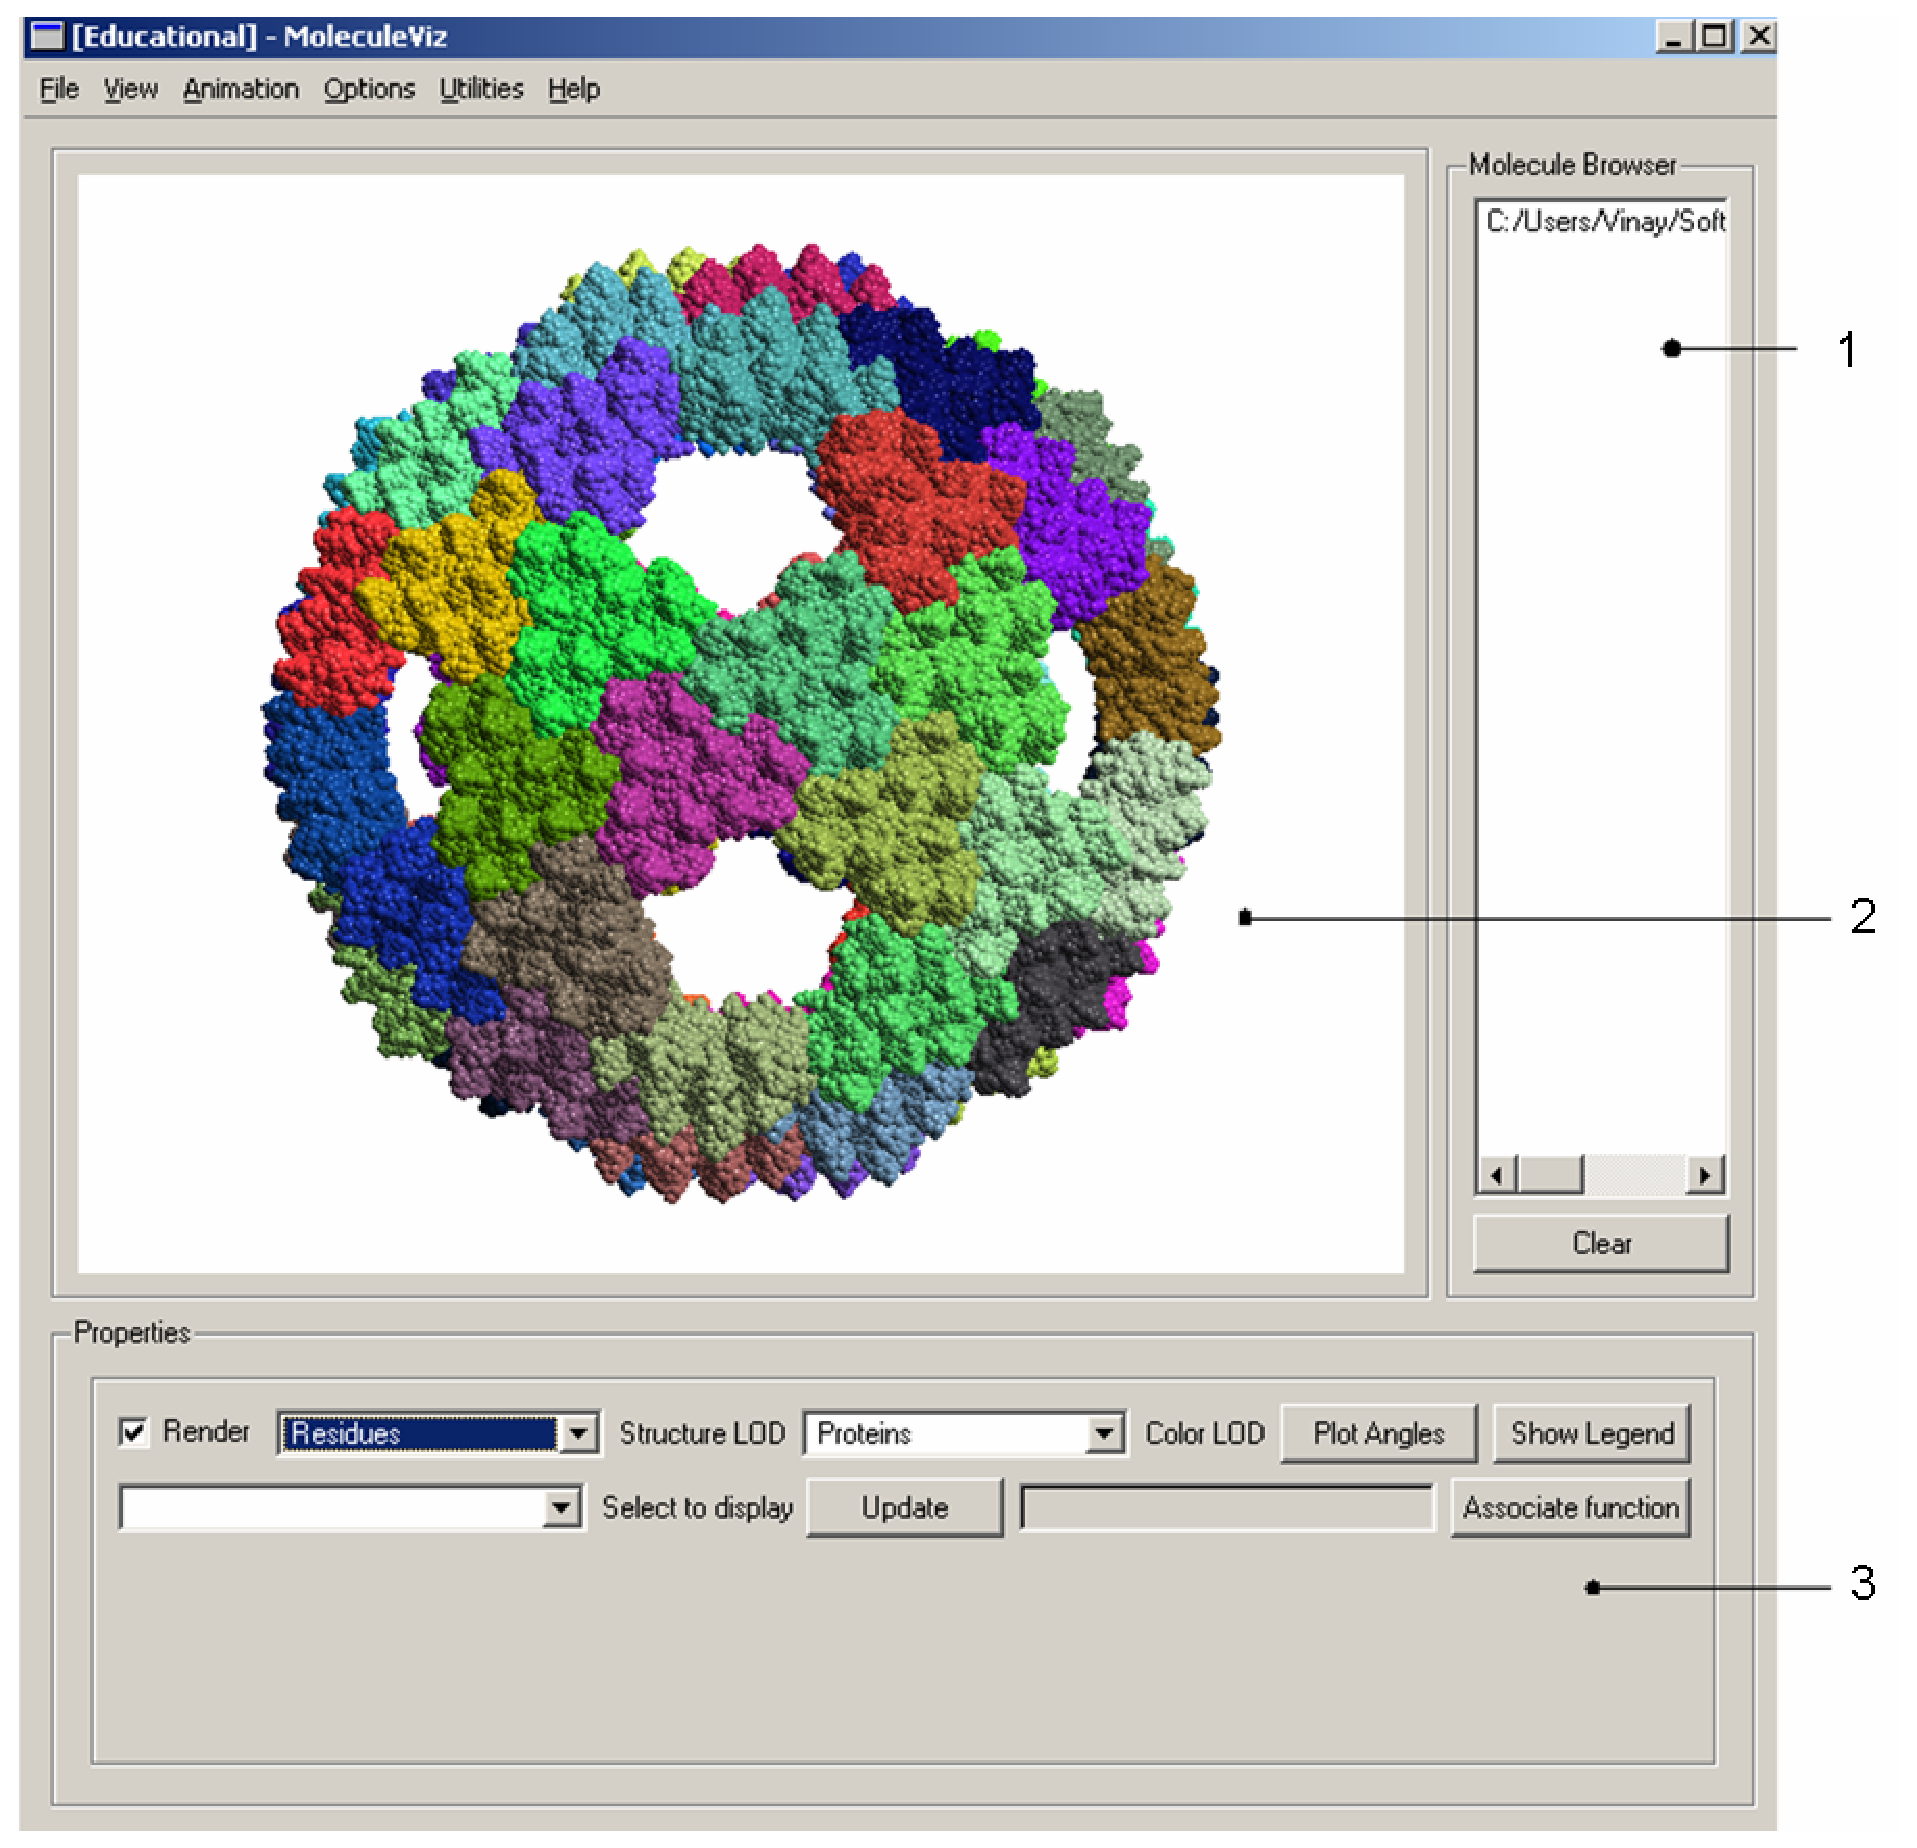
\includegraphics[width=5in]{Images/UserInterface.ps}
\ccaption{The main user interface of \TexMol. In this figure, we
mark the three main regions users should get familiar with: 1.
\emph{Molecule browser} where data sets names are displayed 2.
\emph{Rendering area}, where data is rendered and 3. The
\emph{Properties widget} where the properties of the selected data
set is shown.} \label{figure:userInterface}
\end{figure}

\begin{itemize}

\item Molecule browser. The list of molecules are shown here. The
name is displayed, and if it was left blank on opening the file, the
full filename is shown. The user can select files to either
manipulate it using the properties window or to delete it.

\item The rendering area. This is either in perspective or
orthographic mode, runs using OpenGL and can be either a single or
multiple views.

\item Properties area. Each type of file  (volume, molecule or
surface) has its own unique properties widget which is displayed
here. On selecting a data set from the browser, its corresponding
properties are displayed here.

\end{itemize}


\cchapter{Opening and rendering files}

TexMol reads molecule-specific PDB, PQR files (including simpler
XYZ, XYZR, PTS and a custom GOA formats), volume files (RAWIV, RAWV,
DX, MRC), surface files (RAW, RAWC, RAWN, RAWNC, OBJ, C2C) and a
custom NURBS file. By default, the data set is neither centered to
the view, nor rendered to screen. The user needs
to specifically render the data set after loading it.\\

\warning{If you do not have a good high end graphics card, or if it
is not set up properly to display using Cg, you will not see any
output on the screen. We are in the process of moving to OpenGL
Shading Language.}


\csection{Loading a molecule description file}

We support multiple molecular files. The most commonly used file
formats are PDB \cite{pdb} and PQR \cite{pqr}. We also have simple
file formats to describe general point sets: XYZ (list of centers on
successive lines), XYZR (same, includes radius next to center) and
PTS (similar to XYZ, but first line contains number of centers). The
properties box for molecular data sets is shown in figure
\ref{Figure:MoleculesPropertyBox}. There are two LODs as shown in
the figure, the color LOD and the object LOD.

\begin{figure}
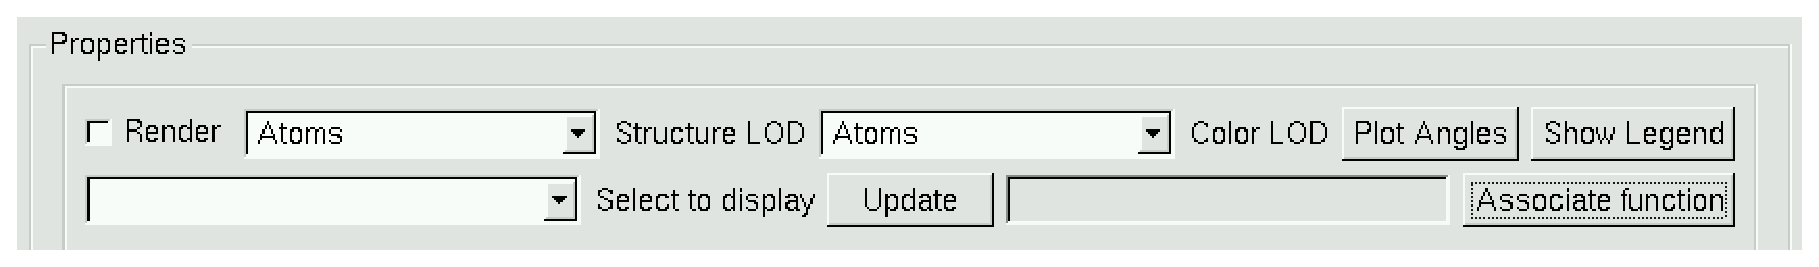
\includegraphics[width=5in]{Images/MoleculeFileProperties.ps}
\ccaption{The \emph{Properties widget} for molecule data sets allows
users to pick their choice of color and structure level of detail to
render. Other functions include associating a volumetric function
with the surfaces color.} \label{Figure:MoleculesPropertyBox}
\end{figure}

\subsection{The static hierarchy for biomolecules}

We use the biochemical hierarchy in our visualizations. For atoms,
we use the CPK model, with van der Waals radii. The colors and
radius used are described in the table in
\emph{elementInformation.h}. Atoms are grouped into residues, which
are approximated by spheres in the structure LOD. Secondary
structures are rendered with imposters like cylinders and helices.
Chains are rendered as a ball-and-stick model.

\begin{itemize}
\item Atoms. The atom sequence is the lowest, or finest level in the
hierarchy to obtain the primary structure of the molecule.

\item Residues. Atoms are grouped into their respective residues.

\item Secondary structures. Residues are grouped in to either
helices or sheets, or into dummy NULL structures.

\item Chains. The secondary structures are collected in to chains.
They form the tertiary structure.

\item Molecule. The highest or coarsest level in the static
hierarchy is the molecule itself.

\end{itemize}

After loading the molecule file, one can select a combination of
color and structure LOD to obtain various visualizations. To open a
PDB or PQR file, follow the steps shown in table
\ref{Table:OpenMoleculeFile}. A simple well known molecule to start
with would be hemoglobin (1A00.pdb), as it has multiple chains and
helices. Some interesting combinations of visualizations would be as
shown in figure \ref{Figure:hemoglobinVisualizations}. Table
\ref{Table:showHelices} explains how one can visualize the helices
in the loaded molecule.

\begin{figure}
     \centering
     \subfigure[Atoms colored with element colors]{
          \label{Figure:hemoglobinVisualizationsa}
          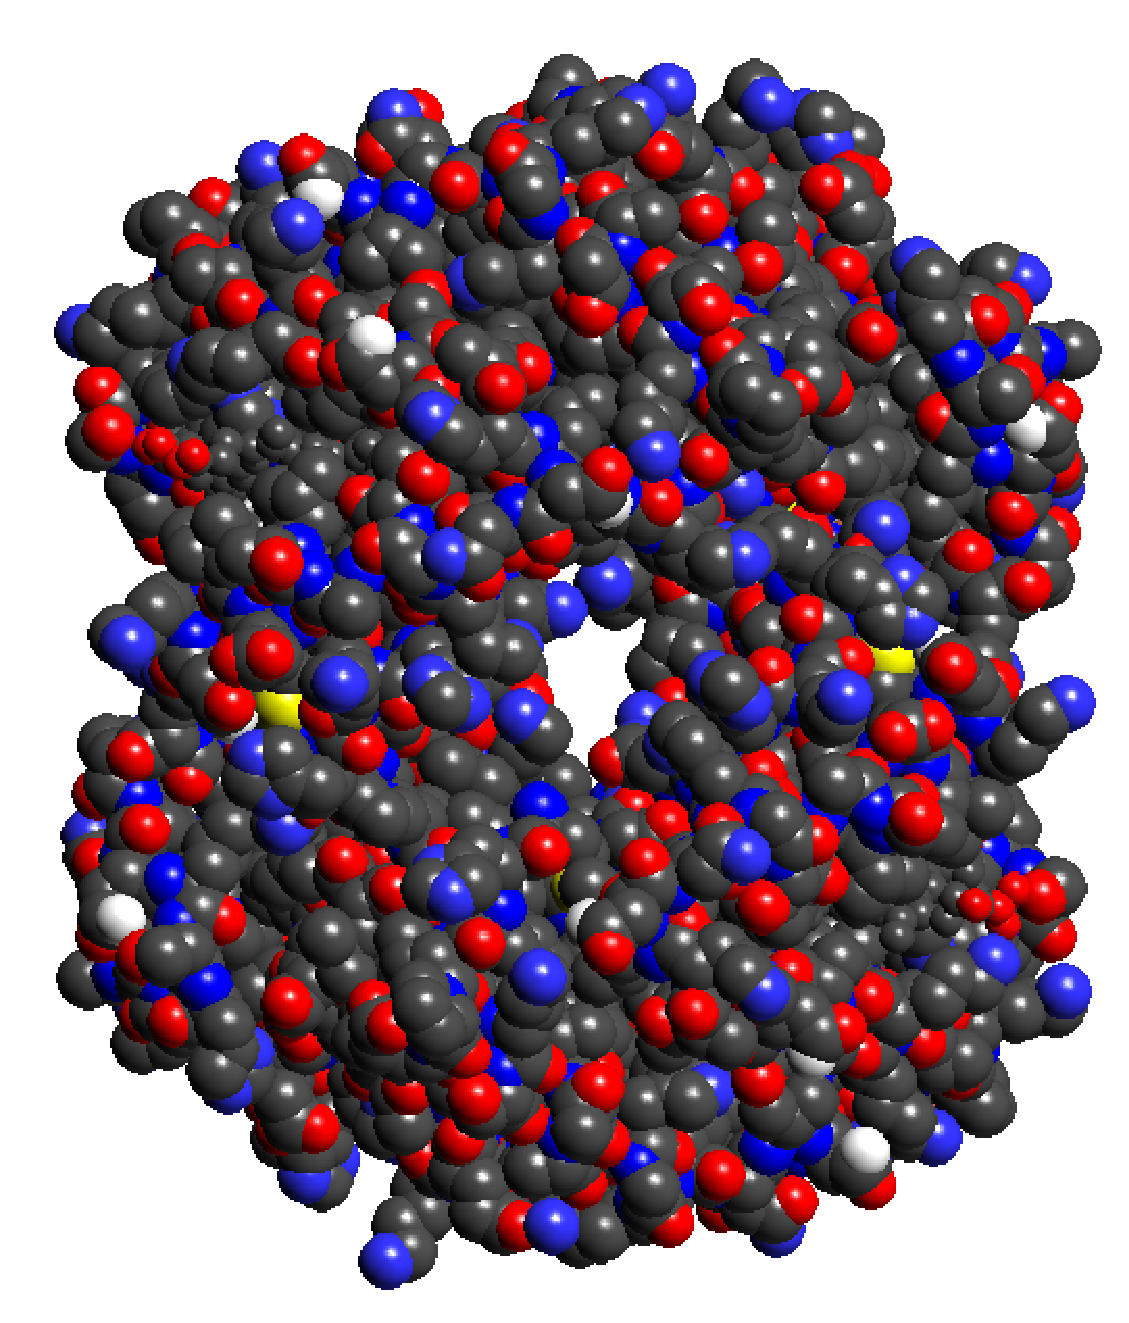
\includegraphics[width=.45\textwidth]{Images/Hemoglobin_Atoms.ps}}
     \hspace{.3in}
     \subfigure[Atoms colored with their respective residues colors]{
          \label{Figure:hemoglobinVisualizationsb}
          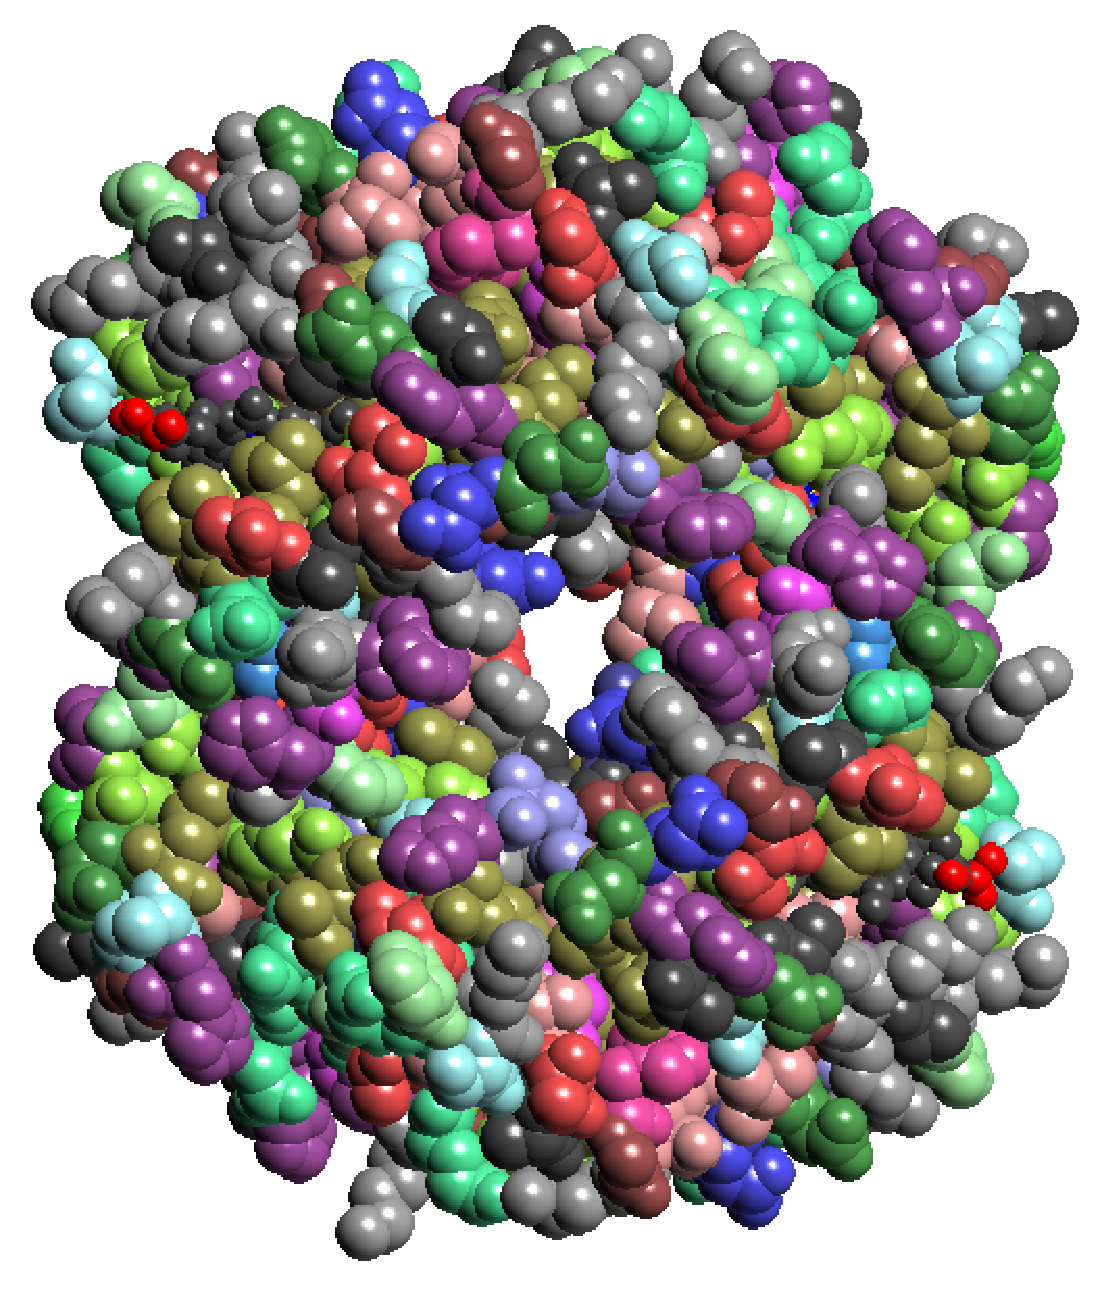
\includegraphics[width=.45\textwidth]{Images/Hemoglobin_atoms_residue_colors.ps}}\\
     \vspace{.3in}
     \subfigure[A coarser model with residues rendered as spheres]{
          \label{Figure:hemoglobinVisualizationsc}
          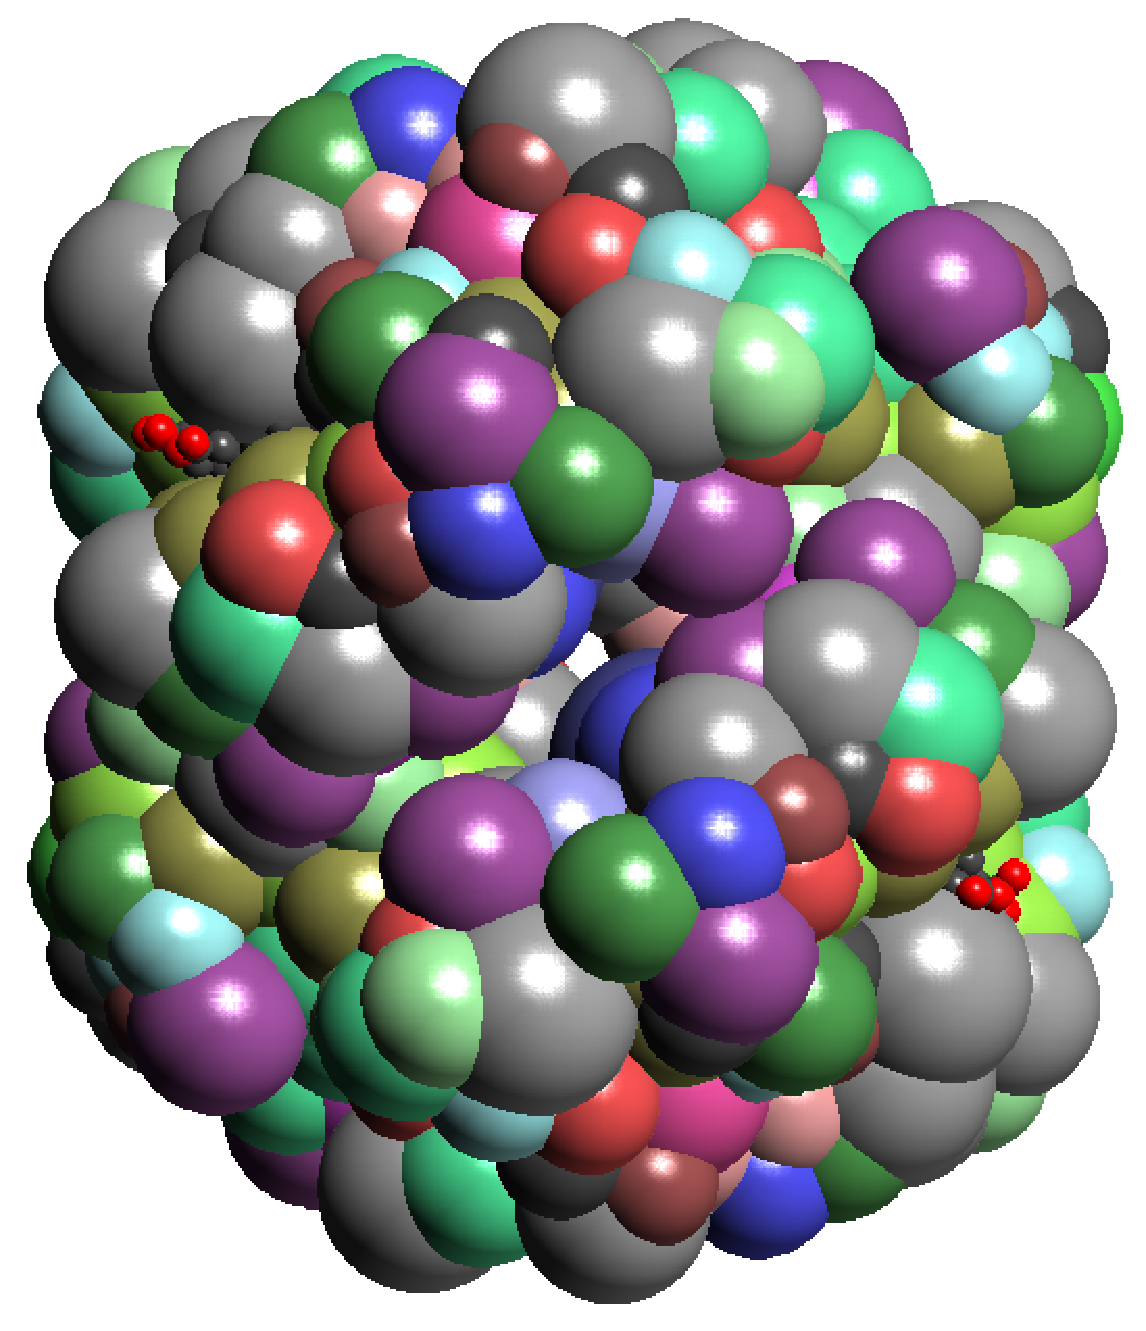
\includegraphics[width=.45\textwidth]{Images/Hemoglobin_Residues.ps}}
     \hspace{.3in}
     \subfigure[Helices forming the secondary structures in the molecule]{
          \label{Figure:hemoglobinVisualizationsd}
          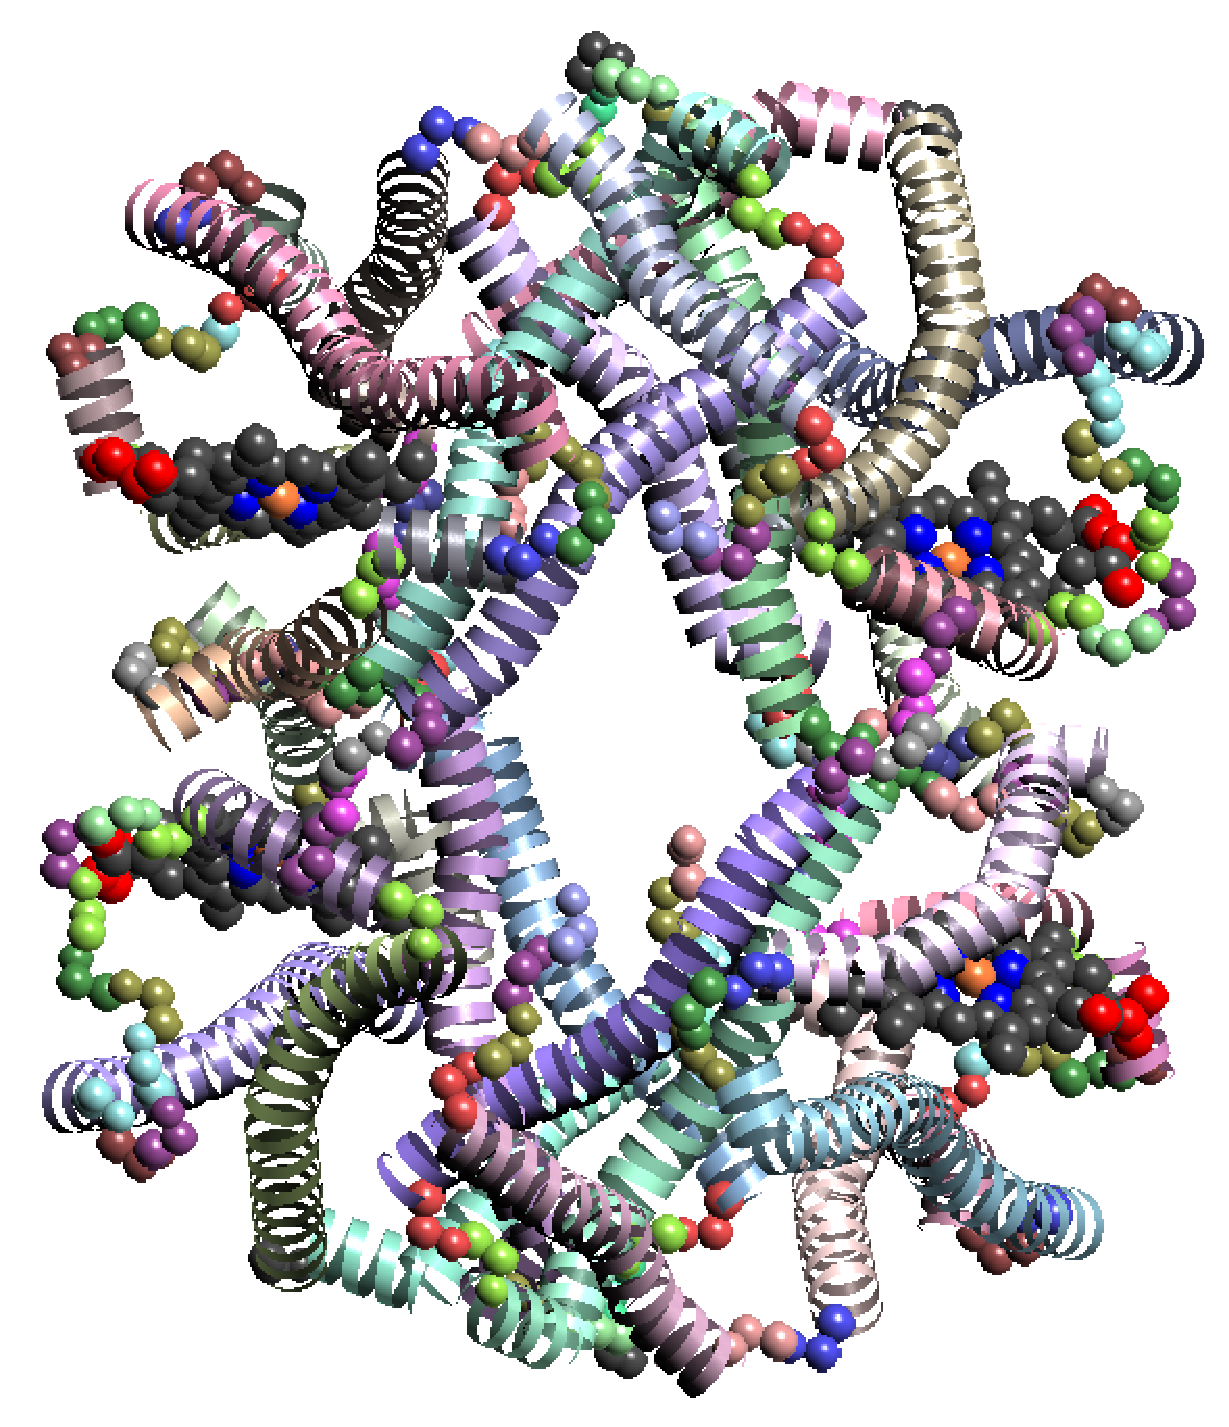
\includegraphics[width=.45\textwidth]{Images/Hemoglobin_ss.ps}}\\
     \caption{Molecules can be rendered at different color and structure level of details.
     Here we show the hemoglobin molecule (1A00.pdb) rendered in 4 different styles.}
     \label{Figure:hemoglobinVisualizations}
\end{figure}

\steps{Loading a molecule}{Table:OpenMoleculeFile}{ \item Select
File - Open from menu bar.
\item Choose a file name by pressing the File button and select a
PDB or PQR file.
\item If you know that you are choosing a isosahedral virus, check the isVirus check box.
\item Press OK to load the file, or Cancel to cancel this action.}

\steps{Visualizing helices in a molecule}{Table:showHelices}{\item
If you have not loaded a molecule, do so by following the steps
outlined in Table \ref{Table:OpenMoleculeFile}. \item Set the
Structure LOD to Secondary structures and the Color LOD to any item.
\item Render the molecule by checking the Render check box. \item If
the molecule is not visible in the current view point, you may need
to zoom out and translate to bring it in to view.}

\csection{Loading volume files}

We currently support four volume files including the scalar RAWIV,
MRC and DX formats, and vector valued RAWV formats. They are both
binary and ascii files and support multiple data types and sizes.
For a complete description, see the file format descriptions on the
CCV web site. To load volume files, follow the same steps as
outlined in table \ref{Table:OpenMoleculeFile}, but select a volume
file instead of a molecule file.

To render volume files and isosurfaces, you need to get familiar
with a widget called a color table, which is user interface for
reading a transfer map. A detailed description for the color table
can be found in the volume rover software user guide.

\csection{Loading surface files}

\warning{Surface files currently supported can be compressed or not.
The uncompressed files can take up to a few minutes to load for very
large meshes.}

 Like volume files, surface files do not need to deal with
molecules. \TexMol currently supports uncompressed (RAW, RAWC, RAWN,
RAWNC and OBJ) and compressed (c2c) surface files. To load any of
these file formats, table \ref{Table:OpenMoleculeFile} can be
followed with the right input file types. Both wireframe and surface
rendering modes are supported. The user can also view both together.
A visualization of the Mache molecule, showing the gorge is shown in
figure \ref{Figure:MACHE}. The OBJ file format is from Alias
Wavefront.

\begin{figure}
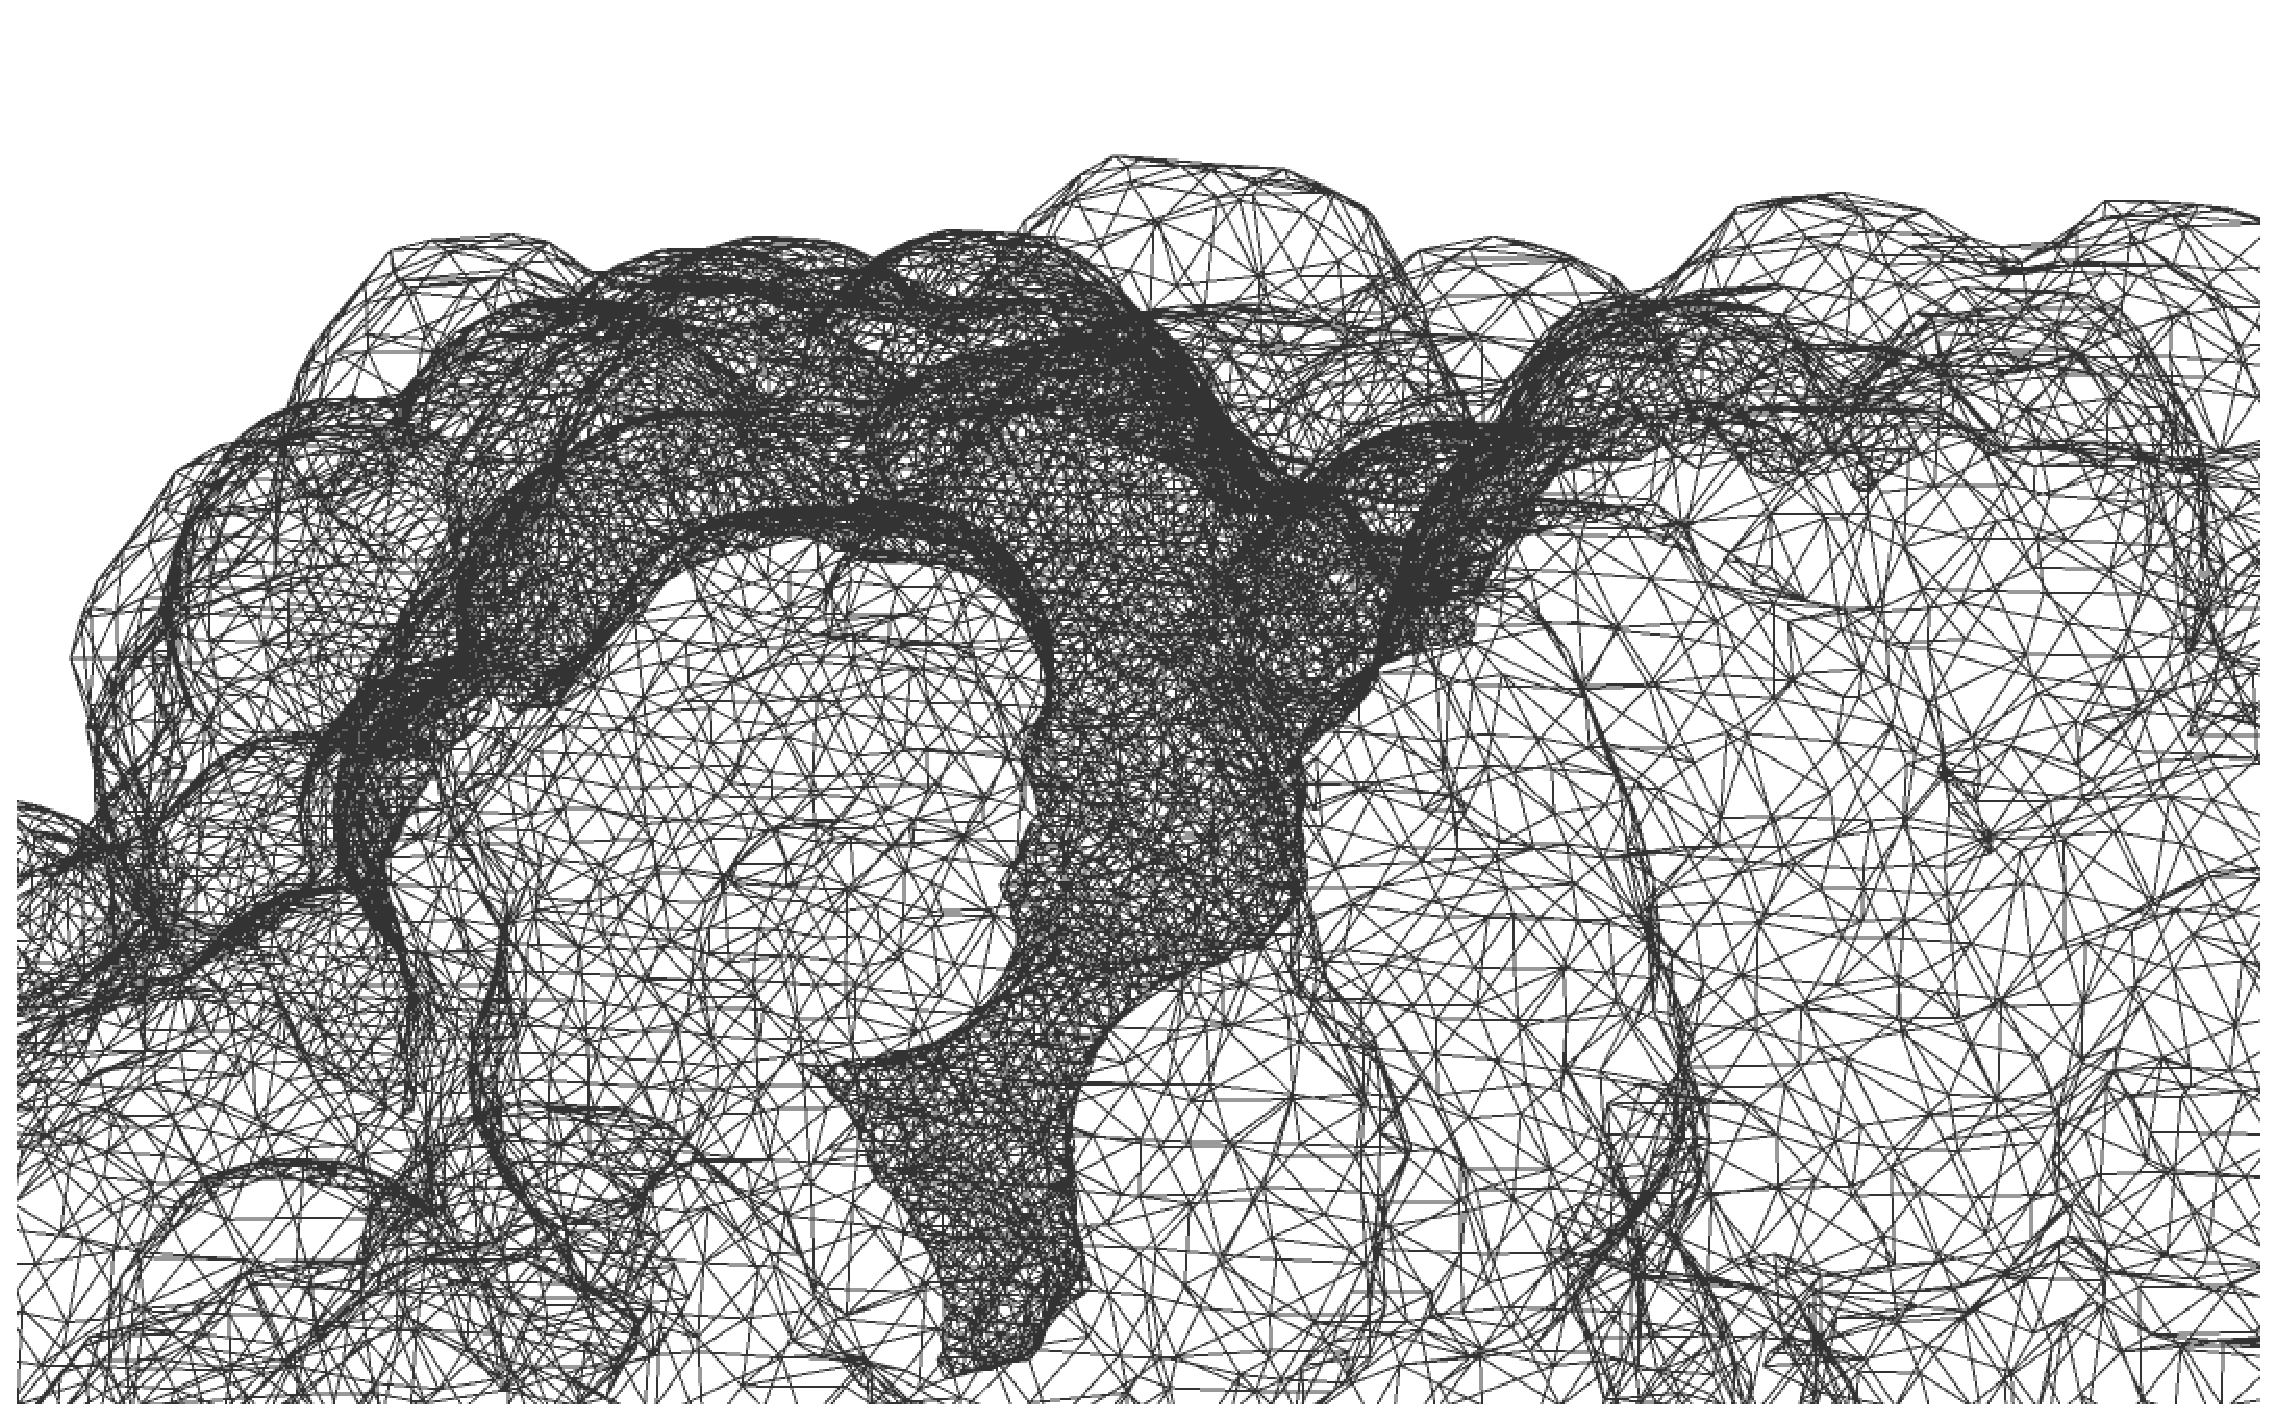
\includegraphics[width=5in]{Images/MacheWireframe.ps}
\ccaption{Wireframe rendering of a mesh, showing a gorge type
feature in the surface of the MACHE molecule.} \label{Figure:MACHE}
\end{figure}


\input{computations}

\cchapter{Scripting and animations}

The computations defined in chapter \ref{Chapter:computations} can
also be performed in batch mode. This is useful when a large number
of files need to be manipulated at once. Two other powerful features
of \TexMol include
\begin{itemize}
\item Scripting.
\item Animation.
\end{itemize}
In this chapter, we will go through simple examples for each of the
above three features.

\csection{Batch-mode calculations}

Electron density, hydrophobicity and curvatures can be estimated
from the command line. The commands are as follows.

\subsection{Electron density and hydrophobicity}

The command line for creating an electron density or hydrophobicity
map is:

\TexMol \textbf{-blur} \param{input molecule file name}
\param{output volume file name} \param{dim1} \param{dim2}
\param{dim3}
\param{density type} \param{colored volume} \param{gaussian
blobbiness}
\param{color} \param{colormap file name} \param{gap}

The different parameters are:

\param{input molecule file name} The full path and name of the input molecule
file.

\param{output volume file name} The full path and name of the output
rawiv or rawv file.

\param{dim1, dim2, dim3} Dimensions of the output volume.

\param{density type} Enter \mm{0} for electron density and \mm{1} for
hydrophobicity.

\param{colored volume} \emph{true} if you want a rawv volume.

\param{gaussian blobbiness} We recommend a value of -2.3 to conform
with previous research and bigger values, say -0.1, to get smoother
shapes representing the volume at much lower resolutions.

\param{color} If the colored volume parameter was true, then we can
either specify either color by structure or provide a color map
file. If we do not provide a color map file, then this parameter is
relevant. \mm{0} stands for atom coloring, \mm{1} for residue,
\mm{2} for secondary structure and \mm{3} for chain coloring.

\param{colormap file name} The molecule can be colored according to
some user defined colors, to perhaps highlight some structure which
cannot be done in the more general method previous described. The
file format for the \emph{colormap file name} is given in the file
format description page from CCV's website.

\param{gap} This should be used sparingly, to provide a gap of empty
space around the requested dimensions. It is best left as \mm{0}.

\subsection{Curvatures}

There are two commands for generating curvatures. One is from a
volume file with a given isovalue, where \TexMol extracts the mesh
where we need to obtain the curvature, and second, where the user
inputs the mesh directly. The two commands in order are:

\TexMol \textbf{-setcurvature} \param{1} \param{input molecule file
name} \param{output volume file name} \param{output mean curvature
file name} \param{output gaussian curvature file name} \param{dim1}
\param{dim2} \param{dim3} \param{gaussian
blobbiness} \param{isovalue} \param{number of grid subdivisions}
\param{maximum function error}\\

\TexMol \textbf{-setcurvature} \param{0} \param{input molecule file
name} \param{input surface file name} \param{output mean curvature
file name} \param{output gaussian curvature file name} \param{dim1}
\param{dim2} \param{dim3} \param{gaussian
blobbiness} \param{number of grid subdivisions}
\param{maximum function error}\\

The various parameters are described below.

\param{0} and \param{1} differentiate between the two calls.

\param{input molecule file name} The full path and name of the input molecule
file.

\param{output volume file name} The full path and name of the output
rawiv or rawv file.

\param{output mean curvature file name} The full path and name of
the output mean curvature file.

\param{output gaussian curvature file name} The full path and name of
the output gaussian curvature file.

\param{dim1, dim2, dim3} Dimensions of the output volume.

\param{gaussian blobbiness} We recommend a value of -2.3 to conform
with previous research and bigger values, say -0.1, to get smoother
shapes representing the volume at much lower resolutions.

\param{number of grid subdivisions} The higher this value, the more
the precomputation and memory requirement. There is a cut off value
around 10 to 20 where you get optimum speed for a given machine.

\param{maximum function error} The maximum allowable function error
while calculating the curvatures.

\warning{While creating curvatures, if we overestimate the value of
grid spacing, we could end up with very high memory usages and may
have to kill the program.}


\csection{Scripting}

\TexMol currently offers a limited but powerful set of functions as
part of its scripting module. This module is available once \TexMol
is run in user interface mode. The parser command window can be
opened from Utilities - script from the main menu bar. Here users
can enter commands, select one or more and execute them. Some of the
commands available are listed below.

\textcolor{BrickRed}{bool} blur(\textcolor{BrickRed}{int} argc,
\textcolor{BrickRed}{char*} argv[]);

\textcolor{BrickRed}{bool} setCurvature(\textcolor{BrickRed}{int}
argc, \textcolor{BrickRed}{char*} argv[]);

\textcolor{BrickRed}{bool}
outGridPositions(\textcolor{BrickRed}{int} argc,
\textcolor{BrickRed}{char*} argv[]);

\textcolor{BrickRed}{bool} classifyPoints(\textcolor{BrickRed}{int}
argc, \textcolor{BrickRed}{char*} argv[]);

\textcolor{BrickRed}{bool} growOut(\textcolor{BrickRed}{int} argc,
\textcolor{BrickRed}{char*} argv[]);

\textcolor{BrickRed}{bool} getSurface(\textcolor{BrickRed}{int}
argc, \textcolor{BrickRed}{char*} argv[]);

\textcolor{BrickRed}{bool} evolve(\textcolor{BrickRed}{int} argc,
\textcolor{BrickRed}{char*} argv[]);

\textcolor{BrickRed}{bool} writePDB(\textcolor{BrickRed}{int} argc,
\textcolor{BrickRed}{char*} argv[]);

\textcolor{BrickRed}{bool} writeGOA(\textcolor{BrickRed}{int} argc,
\textcolor{BrickRed}{char*} argv[]);

\textcolor{BrickRed}{bool} depthColor(\textcolor{BrickRed}{int}
argc, \textcolor{BrickRed}{char*} argv[]);

\textcolor{BrickRed}{bool}
printPDBInformation(\textcolor{BrickRed}{int} argc,
\textcolor{BrickRed}{char*} argv[]);

\textcolor{BrickRed}{bool}
getMaxDistanceFromPoint(\textcolor{BrickRed}{int} argc,
\textcolor{BrickRed}{char*} argv[]);

\textcolor{BrickRed}{bool} addNewDataSet(\textcolor{BrickRed}{int}
argc, \textcolor{BrickRed}{char*} argv[],
\textcolor{BrickRed}{MoleculeVizMainWindow} *mWindow );

\textcolor{BrickRed}{bool} splitView(\textcolor{BrickRed}{int} argc,
\textcolor{BrickRed}{char*} argv[],
\textcolor{BrickRed}{MoleculeVizMainWindow} *mWindow );

\textcolor{BrickRed}{bool} deleteData(\textcolor{BrickRed}{int}
argc, \textcolor{BrickRed}{char*} argv[],
\textcolor{BrickRed}{MoleculeVizMainWindow} *mWindow );


\textcolor{BrickRed}{bool} deletePrevData(\textcolor{BrickRed}{int}
argc, \textcolor{BrickRed}{char*} argv[],
\textcolor{BrickRed}{MoleculeVizMainWindow} *mWindow );


\textcolor{BrickRed}{bool} deleteAllData(\textcolor{BrickRed}{int}
argc, \textcolor{BrickRed}{char*} argv[],
\textcolor{BrickRed}{MoleculeVizMainWindow} *mWindow );


\textcolor{BrickRed}{bool} setVisible(\textcolor{BrickRed}{int}
argc, \textcolor{BrickRed}{char*} argv[],
\textcolor{BrickRed}{MoleculeVizMainWindow} *mWindow );


\textcolor{BrickRed}{bool} setVisiblePrev(\textcolor{BrickRed}{int}
argc, \textcolor{BrickRed}{char*} argv[],
\textcolor{BrickRed}{MoleculeVizMainWindow} *mWindow );


\textcolor{BrickRed}{bool} saveImage(\textcolor{BrickRed}{int} argc,
\textcolor{BrickRed}{char*} argv[],
\textcolor{BrickRed}{MoleculeVizMainWindow} *mWindow );


\textcolor{BrickRed}{bool} setGridVisible(\textcolor{BrickRed}{int}
argc, \textcolor{BrickRed}{char*} argv[],
\textcolor{BrickRed}{MoleculeVizMainWindow} *mWindow );



\csection{Animations}

This module is mainly useful for making movies. Animations can be
saved as a sequence of images in \TexMol. We allow the user to load
a data set, render it and transform the view point, and save
trajectories and play it back. There are actually two steps in the
animation process.

\begin{enumerate}
\item Create and save a trajectory.
\item Save the animation based on a trajectory.
\end{enumerate}

\subsection{Creating a trajectory}
\label{subsection:CreateTrajectory}

Data sets can be quite large, making them hard to interact with.
Hence, it is sometimes useful to save a trajectory using a low
resolution data set and later use it to render a large data set in
high resolution. In order to create the trajectory it is useful to
have a low resolution data set which the user can comfortably
rotate, zoom and translate interactively. To save a trajectory,
follow the procedure outlined in table \ref{Table:Trajectory}

\steps{Creating and saving a trajectory}{Table:Trajectory}{\item
Load and display the data set or set of data sets you want to create
a movie of.
\item Use the mouse to move them into the correct starting viewing
position. \item Click Animation, Start recording from the menu bar.
\item Enter and save the file name of the trajectory file. It does
not require any specific file extension. \item On pressing OK, the
recording is on. Any mouse movement in the rendering area is saved
in to the file, along  with the time. \item Once you are done with
transforming the data, click Animation, Stop recording in the menu
bar. \item You can see if the trajectory was satisfactory by playing
it back by clicking on Animation, Playback animation from the menu
bar.}

\subsection{Saving animations}

Before you can save a sequence of images, you need to create a
trajectory as described in section
\ref{subsection:CreateTrajectory}.


\steps{Saving an animation}{Table:SavingAnimations}{ \item Load the
high resolution data sets to save.
\item keep the screen resolution and window size as high as
required.
\item Open the trajectory file by selecting Animation, Record
animation from the menu bar. \item \TexMol will automatically begin
to replay the trajectory and save images.}

\warning{Disable the screensaver as saving images in high resolution
can take a long time. We also interpolate between mouse movements
using linear interpolation to get better smoothness, causing the
movie to be longer than expected.}


\chapter*{Acknowledgements}\normalsize\addcontentsline{toc}{chapter}{Acknowledgements}

\TexMol was developed by Vinay K Siddavanahalli under Prof
Chandrajit Bajaj. Some of the other contributors include

\begin{itemize}
\item Peter Djeu
\item Anthony Thane
\item John Wiggins
\item Xiaoyu Zhang
\end{itemize}


\begin{thebibliography}{99}
  \addcontentsline{toc}{chapter}{Bibliography}
\bibitem{texmol} Chandrajit Bajaj, Peter Djeu, Vinay Siddavanahalli and Anthony Thane {{\bf \TexMol}: Interactive Visual Exploration of Large Flexible Multi-component Molecular
Complexes} IEEE Visualization 2004.
\bibitem{pdb} H.M. Berman, J. Westbrook, Z. Feng, G. Gilliland, T.N. Bhat, H.
Weissig, I.N. Shindyalov, P.E. Bourne: The Protein Data Bank.
Nucleic Acids Research, 28 pp. 235-242 (2000).
\bibitem{pqr}Todd J. Dolinsky, Jens E. Nielsen, J. Andrew McCammon, and Nathan
A. Baker: PDB2PQR: an automated pipeline for the setup of
Poisson�Boltzmann electrostatics calculations.  Nucleic Acids Res.
2004 July 1; 32
\bibitem{bajaj06fast}Chandrajit Bajaj and Vinay Siddavanahalli,  Fast Error-bounded
Surfaces and Derivatives Computation for Volumetric Particle Data,
ICES Report 06-03, January 2006.
\end{thebibliography}



\include{index}
  \addcontentsline{toc}{chapter}{Index}

\end{document}
